\documentclass[11pt]{article}

% --- Packages ---
\usepackage[usenames, dvipsnames]{color} % Cool colors
\usepackage{enumerate, amsmath, amsthm, amssymb, mathrsfs, algorithm, algpseudocode, fontawesome, pifont, subfig, fullpage, csquotes, dashrule, tikz, bbm, booktabs, bm, hyperref}
\usepackage[framemethod=TikZ]{mdframed}
\usepackage[numbers]{natbib}
\usepackage[normalem]{ulem}

% --- Misc. ---
\hbadness=10000 % No "underfull hbox" messages.
\setlength{\parindent}{0pt} % Removes all indentation.

% -- Commands --
% COMMANDS:
% - bigmid: Dynamically sized mid bar.
% - spacerule: add a centered dashed line with space above and below
% - \dbox{#1}: Adds a nicely formatted slightly grey box around #1
% - \begin{dproof} ... \end{dproof}: A nicely formatted proof. Use \qedhere to place qed
% - \ddef{#1}{#2}: Makes a definition (and counts defs). #1 goes inside parens at beginning, #2 is actual def.
% - \begin{dtable}{#1} ... \end{dtable}: Makes a minimalist table. #1 is the alignment, for example: {clrr} would be a 4 column, center left right right table.

% Dynamically sized mid bar.
\newcommand{\bigmid}{\mathrel{\Big|}}


% ---- Colors and Notes ----
\definecolor{dblue}{RGB}{98, 140, 190}
\definecolor{dlblue}{RGB}{216, 235, 255}
\definecolor{dgreen}{RGB}{124, 155, 127}
\definecolor{dpink}{RGB}{207, 166, 208}
\definecolor{dyellow}{RGB}{255, 248, 199}
\definecolor{dgray}{RGB}{46, 49, 49}

% TODO
\newcommand{\todo}[1]{\textcolor{red}{TODO: #1}}
\newcommand{\dnote}[1]{\textcolor{dblue}{Dave: #1}}

% URL
\newcommand{\durl}[1]{\textcolor{dblue}{\underline{\url{#1}}}}

% Circled Numbers
\newcommand*\circled[1]{\tikz[baseline=(char.base)]{\node[shape=circle,draw,inner sep=0.7pt] (char) {\footnotesize{#1}};}}
% From: http://tex.stackexchange.com/questions/7032/good-way-to-make-textcircled-numbers

% Under set numbered subset of equation
\newcommand{\numeq}[3]{\underset{\textcolor{#2}{\circled{#1}}}{\textcolor{#2}{#3}}}

% ---- Abbreviations -----
\newcommand{\tc}[2]{\textcolor{#1}{#2}}
\newcommand{\ubr}[1]{\underbrace{#1}}
\newcommand{\uset}[2]{\underset{#1}{#2}}
\newcommand{\eps}{\varepsilon}

% Typical limit:
\newcommand{\nlim}{\underset{n \rightarrow \infty}{\lim}}
\newcommand{\nsum}{\sum_{i = 1}^n}
\newcommand{\nprod}{\prod_{i = 1}^n}

% Add an hrule with some space
\newcommand{\spacerule}{\begin{center}\hdashrule{2cm}{1pt}{1pt}\end{center}}

% Mathcal and Mathbb
\newcommand{\mc}[1]{\mathcal{#1}}
\newcommand{\indic}{\mathbbm{1}}
\newcommand{\bE}{\mathbb{E}}

\newcommand{\ra}{\rightarrow}
\newcommand{\la}{\leftarrow}

% ---- Figures, Boxes, Theorems, Etc. ----

% Basic Image
\newcommand{\img}[1]{
\begin{center}
\includegraphics[\width=0.6\textwidth]{#1}
\end{center}}

% Put a fancy box around things.
\newcommand{\dbox}[1]{
\begin{mdframed}[roundcorner=4pt, backgroundcolor=gray!5]
\vspace{1mm}
{#1}
\end{mdframed}
}

%  --- PROOFS ---

% Inner environment for Proofs
\newmdenv[
  topline=false,
  bottomline=false,
  rightline = false,
  leftmargin=10pt,
  rightmargin=0pt,
  innertopmargin=0pt,
  innerbottommargin=0pt
]{innerproof}

% Proof Command
%\newenvironment{dproof}{\begin{proof} \text{\vspace{2mm}} \begin{innerproof}}{\end{innerproof}\end{proof}\vspace{4mm}}
\newenvironment{dproof}[1][Proof]{\begin{proof}[#1] \text{\vspace{2mm}} \begin{innerproof}}{\end{innerproof}\end{proof}\vspace{4mm}}


% Dave Definition
\newcounter{DaveDefCounter}
\setcounter{DaveDefCounter}{1}

\newcommand{\ddef}[2]
{
\begin{mdframed}[roundcorner=1pt, backgroundcolor=white]
\vspace{1mm}
{\bf Definition \theDaveDefCounter} (#1): {\it #2}
\stepcounter{DaveDefCounter}
\end{mdframed}
}

% Block Quote
\newenvironment{dblockquote}[2]{
\begin{blockquote}
#2
\vspace{-2mm}\hspace{10mm}{#1} \\
\end{blockquote}}

% Algorithm
\newenvironment{dalg}[1]
{\begin{algorithm}\caption{#1}\begin{algorithmic}}
{\end{algorithmic}\end{algorithm}}




% Dave Table
\newenvironment{dtable}[1]
{\begin{figure}[h]
\centering
\begin{tabular}{#1}\toprule}
{\bottomrule
\end{tabular}
\end{figure}}

% For numbering the last of an align*
\newcommand\numberthis{\addtocounter{equation}{1}\tag{\theequation}}

\DeclareMathOperator*{\argmin}{arg\,min}
\DeclareMathOperator*{\argmax}{arg\,max}

\newtheorem{conjecture}{Conjecture}[section]
\newtheorem{remark}{Remark}[section]
\newtheorem{theorem}{Theorem}[section]
\newtheorem{corollary}{Corollary}[theorem]
\newtheorem{lemma}[theorem]{Lemma}
\newtheorem{assumption}{Assumption}


\title{IACAP 2019 Notes \\ \Large{Mexico City, Mexico}}
\author{David Abel\footnote{\durl{http://david-abel.github.io}} \\ \durl{david_abel@brown.edu}}
\date{June 2019}

\begin{document}
\maketitle
\tableofcontents
\newpage


This document contains notes I took during the events I managed to make it to at (my first) IACAP, in Mexico City, Mexico. Please feel free to distribute it and shoot me an email at \durl{david_abel@brown.edu} if you find any typos or other items that need correcting. 


\section{Conference Highlights}


% ------------
% -- Sunday --
% ------------
\newpage
\section{Wednesday June 5th}
Today we'll have talks focusing

\subsection{Fiona McEvoy on AI-Driven Behavior Change}

{\bf Goal:} recommendations for future research on {\it decision guidance} algorithms (not decision-making algorithms). \\

$\ra$ Example: google results based on clicks/habits, recommendations systems. \\

``Nudge": any aspect of a system/intervention that alters people's behavior in a predictable way without forbidding any options or significantly changing economic incentives. Think: bench with bars on it vs. a sign. \\

{\bf Two Decision-Making Systems:} System 1 (automatic/intuition), and System 2 (rational thinking). ``Nudge" is making use of System 1. \\

\ddef{Hypernudging}{A feedback loop online that contributes heavily to how individuals make decision.}

$\ra$ Data collection about decisions and actions. \\

{\bf Point:} Hypernudging has been accused of manipulation. \\

Q: Which features keep nudges consistent with autonomous human decision-making, and which force them to be manipulative? \\

Hypothesis: the more imersive an environment is, the more they can manipulate individuals. \\

\ddef{Autonomy}{Two notions: 1) the {\it opportunity} for autonomy; Mill's freedom from manipulation, and 2) capacity for autonomy; I should be able to pursue my goals.}

One group: The environment is full of non-rational influences. So, even our most rational decisions fall out of non-rational effects. Therefore, it must be permissible to shape the choice environment. \\

$\ra$ Distinction: shaping environment vs distorting! ``Shape" is \dnote{I missed it, something like ``A intends to Y, based on Z"}, vs. distort: ``A intends to do X". \\


Features of ethically-permissible nudges:
\begin{itemize}
    \item A range of options from which to choose
    \item Can make a decision that differs from the preferences of the individual.
    \item Environment is non-deceptive/distorting/subliminal.
\end{itemize}

Three case studies:
\begin{enumerate}
    \item Online (based on Karen Yeung's work on hypernudges~\cite{yeung2017hypernudge}).
    
    $\ra$ Yeung says most online systems are manipulative in the sense that people are coerced into making non-rational decisions.
    
    \item Voice Controlled IoT: Whoever controls these has immense power: company that makes these software/hardware systems gets to choose a lot of things for you (which music service you use, shopping platform, and so on).
    
    $\ra$ Relationship between IoT/voice systems and people is becoming richer and more complex. Relationships/sensitivity develops, which masks the fact that these items are commercial entities.
    
    \item Virtual/Augmented Reality: New frontier -- nudges/distortion possible by visual/3d construction of avatars, lots of opportunity to manipulate users through the environment. \\
    
    $\ra$ Example: put elementary school kids into a VR environment, and they {\it remembered} the experience (1-2 weeks later) as a real experience (not as VR?).
    
\end{enumerate}

By the nature of all three environments, there is heavy psychological potency to manipulate users. \\

Wired: ``AR will spark the next big tech platform." $\ra$ Claim: we will use AR as the next frontier.

\spacerule

\subsection{Karen Gonzalez-Fernandez on Logic
and Heuristics in Cognitive Psychology}

Logic and heuristics have a long history: heuristics tends to be linked to the process of discovery, particularly under uncertainty and economical considerations. Conversely, logic is about deduction and certainty. \\

Q: Should logic and heuristics both be considered as part of the norms of reasoning in people? \\

{\bf Goal:} Show how logic and heuristics are understood as criteria of rationality. \\

Q: What is the role of logic/heuristics in rationality in cognitive psychology?\\

Proposal 1: ``To be rational is to reason in accordance with principles of reasoning that are based on rules of logic, probability and so forth....such rules are normative principles of reasoning"~\cite{stein1996without}. \\

Proposal 2: heuristics are ``strategies that allos us to make plausible inferences econmizing cognitive resources". \\

$\ra$ Kahneman and Tversky~\cite{kahneman2013prospect}: two systems of reasoning.
\begin{enumerate}
    \item System 1: intuitive system
    \item System 2: rational system.
\end{enumerate}

$\ra$ Heuristics appear in judgments of system 1 because they are more accessible. \\

$\ra$ Heuristics produce {\bf bias} and must be studied mainly to overcome/strategize w.r.t. systematic errors we make. \\

{\bf Gigerenzer:} proposal for ecological rationality~\cite{todd2012ecological}. In ``small worlds" only classical logics an be applied. In ``large worlds", logic can't be applied, so we need heuristics.

$\ra$ Can develop either descriptive models or normative models of heuristics. \\

{\bf Proposal:} Logic vs. heuristics as a criterion of rationality. Consider the following properties:
\begin{dtable}{ll}
{\bf Logic}&{\bf Heuristics} \\
\midrule
Logical Omniscience& Lose valid inferences \\
Infallibility& Fallibility \\
Consistency& Inconsistency \\
Context-free rules& Rules influenced by context\\
No constraints& Limitations of time/memory \\
\end{dtable}

$\ra$ Takeaway: logic and heuristics are in conflict with one another. \\

$\ra$ But, from recent work in AI, perhaps we can find a more cooperative model that incorporates both strategies. Some proposals define an algorithm as logic w/ control, that unifies aspects of both approaches. \\

{\bf Conclusion:} Logic and heuristics can cooperate. Take Gillies proposal that Inference = Logic + control, we can:
\begin{enumerate}
    \item Introduce non-classical logics
    \item Find a better understanding of processes we make when we reason in ordinary life and inside scientific methodology.
    \item Open Problem (for psychologists): Why should we maintain classical logics as a paradigm for rationality? Should we include non-classical logics in our theories of rationality?
    \item Open Problem (for philosophers): What are we doing when we do logic? How should we understand the relationship between logic and reasoning?
\end{enumerate}

\spacerule



\subsection{Keynote: Alexandru Baltag on The Topology of Surprise}

Q: Knowing the world: Can I ever know the state of the world? \\

A: Well, it depends! On three things:
\begin{enumerate}
    \item The actual world: some worlds are knowable, some not.
    \item What can I observe? Topology of observable evidence.
    \item Background information: are we given any prior knowledge?
\end{enumerate}

$\ra$ Knowability of the world sounds metaphysical and unapplied. But, in a state-space formalism, the state of the world is an abstraction: the most refined description of the world that is relevant for the given purposes. \\

$\ra$ This description {\it consists of the answer to relevant questions}. \\

\dbox{Central Question: is it possible to learn the answer to some (relevant) question, given enough observable evidence.}

Consider the following paradox:

\ddef{Surprise Exam Paradox}{A student know the date of an exam is next week. Doesn't know which day. \\

Teacher announces that the exam's date will be a surprise: even in the evening before the exam, the student will not be sure that the exam is tomorrow. (also all participants can't lie).}

But, applying backwards induction: if the announcement is true, then the test cannot take place any day of the week! So, the test cannot be a surprise and the student dismisses the announcement. But then, the test will be a surprise! Paradox. \\

Note that there are multiple interpretations here: the student might not be able to eliminate Thursday (and the rest of the days, only Friday). That is:
\begin{enumerate}
    \item Non-self-referential interpretation: teacher meant ``you wouldn't know in advance the day of the exam, without any help from me (if you are not using even the information that I am announcing now).
    
    $\ra$ Thus, the elimination process stops here.
    
    \item Self-referential interpretation (most common): teacher meant ``you will not know in advance the exam day, period, even after hearing this announcement.
    
    $\ra$ But, this version leads to a paradox (a non-lying teacher can't answer the question ``after hearing this announcement, will the exam still be a surprise?" five times (``no", specifically), and avoid contradiction.
\end{enumerate}


\ddef{Topology}{A topology on a set $\mc{X}$ is given by a family $\mathbb{T} \subseteq P(\mc{X})$, or ``states": possible descriptions of the actual world.}

So: the set of possible worlds is defined by the space $\mc{X}$. \\

$\ra$ Open sets represent the agent's evidence about the world: at world $x \in \mc{X}$, every open set $\mc{U} \in \mathbb{T}$ with $x \in \mc{U}$ is a piece of evidence. \\

Two interpretations: 1) evidence in hand (topology of actual evidence), and 2) evidence out there (topology of potential evidence). \\

Q: Why a topology? \\

A: Start with properties of the world that are directly observable, they form a topological basis. \\

Typical assumptions:
\begin{itemize}
    \item CS/Econominists tend to assume that the topology given is a {\it partition} of the state space $\mc{X}$.
    
    $\ra$ Assumes absolute certainty.
    
    \item Others tend to latch onto {\it potential} evidence, which leads to making no restrictions on the topologies.
\end{itemize}

Setting: multiple agents, multiple perspectives. This requires multiple topologies. \\

Some definitions:
\begin{enumerate}
    \item Neighborhood of a point $x \in \mc{X}$ is  any open set $\mc{U}$ where $x \in \mc{U}$.
    \item Interior point of a set $\mc{A} \subset \mc{X}$ is a point $x$ such that there is a neighborhood of $x$ where $\mc{U} \subseteq \mc{A}$.
    \item A limit point of a set A is a point $x \in \mc{X}$ s.t. every neighborhood of $x$ contains a point $y \in \mc{A}$ with $y \neq x$.
    \item Interior of A is the set of all its interior points:
    \[
    Int(A) = \{x \in \mc{X} \mid \exists U \in \mathbb{T}(x \in \mc{U} \subseteq \mc{A}\}
    \]
    \item Closure of $A$ is:
    \[
    Cl(\mc{A}) = \{x \in \mc{X} \mid \forall U \in \mathbb{T}(x \in \mc{U} \ra \mc{U} \cap \mc{A} \neq \emptyset\}
    \]
    \item The (Cantor) derivative of A is the set of its limits points:
    \[
    d(\mc{A}) := \{x \in \mc{X} \mid \forall \mc{U} \in \mathbb{T}(x \in \mc{U} \ra (\mc{U} - \{x\})\cap A \neq \emptyset\}
    \]
\end{enumerate}

Note: the interior satisfies the dual axioms, corresponding to a modal system (S4):
\begin{align}
    &Int(\mc{X}) = \mc{X}, &Int(\mc{A}) \subseteq \mc{A} \\
    &Int(\mc{A} \cap \mc{B}) = Int(\mc{A}) \cap Int(\mc{B}), &Int(Int(\mc{A})) = Int(\mc{A}).
\end{align}

Epistemic interpretation: captures main properties of a natural concept of knowledge or knowability (based roughly on the modal system S4). \\


Important Distinction: 1) you know/do not know, vs. 2) you can know/cannot know. \\

Example topologies:
\begin{enumerate}
    \item Complete ignorance: the trivial topology $\mathbb{T} = \{\emptyset, \mc{X}\}$.
    \item Omniscience (god): $\mathbb{T} = P(\mc{X}) = \{\mc{Y} \mid \mc{Y} \subseteq \mc{X}\}$
    \item Knowledge based on measurements of points on a line.
\end{enumerate}

So far: we have a proper definition of knowledge and knowability. Let us return to the question: \\

Q: Is the actual state of the world known? \\

A: Depends on evidence. Suppose background information is given by a subset $\mc{A} \subseteq \mc{X}$ of a topological space. \\

$\ra$ Suppose: actual world $x$ belongs to $\mc{A}$. Then, I can know actual world $x$ iff $x$ is isolated in $A$, that is, iff $\{x\} = \mc{U} \cap \mc{A}$ for some open set $\mc{U} \in \tau_\mc{X}$.\\

{\bf Example:} Policeman and the Speeding Car.
\begin{itemize}
    \item Policeman uses a radar with accuracy $\pm$ 2 mph to determine whether the car is speeding in a 50mph zone.
    \item Radar shows 51 mph.
    \item $\mc{X} = (0, \infty)$ is the set of possible worlds where we assume the car is known to be moving.
    \item The property ``speeding" is knowable, but it is now known in this context.
\end{itemize}

{\bf Example:} Teacker marks a point $x$ on a real line $R$. Announces that the point is in the set:
\begin{align}
A = &\{0\}\ \cup OR\\
&\{\frac{1}{n} : n \in \mathbb{N}, n \geq 2\}\ OR \\ &\{\frac{1}{n} + \frac{1}{n^m} : n,m \in \mathbb{N}_{\geq 2}\}\ OR\\
&[1,2].
\end{align}

Q: Can the student know the position? Depends on further measurements, their accuracy, and so on. \\

$\ra$ We can bury a surprise exam paradox in here, too. \\

Let's revisit a topological epistemic analysis of the surprise exam paradox: what is the potential evidence in this context? \\

Under the self-referential view, we can recreate the paradox. The topological analysis gave us some justification as to {\it why} this is a paradox: the only perfect subset of $\mc{A}$ is the empty set! \\

Multi-agent example: Two numbers, one on each of two agents' foreheads. The numbers are off by one. \\

$\ra$ Ask each agent: do you know the number on your head? First time: no! Ask again: no! ask again: yes! Can use Cantor's derivative method to repeatedly eliminate possible worlds until $x$ is known (the true state of the world).
\spacerule





\subsection{David Fernandez-Duque on Stratified Evidence Logic}

Example: Alice wants to know if the movie ``Roma" by Alfonso Cuaron is a good movie. She asks her chatbot, Bot. Bot decides that wikipedia and rotten tomatoes are not sufficient for answering Alice's question. \\

Bot does conclude that an oscar nomination and a rotten tomatoes score of 90\% or higher are sufficient to answer Alice's question. \\

$\ra$ Both can only answer her question with $N = 2$ pieces of evidence. But what if $N$ is really large? $N > 10,000$? \\

{\bf Goal:} Present a logical framework in which the amount of evidence needed to conclude a new belief can be explicitly counted in order to model {\it bounded rationality}. \\

\ddef{Evidence Models}{An evidence model consists of:
\begin{enumerate}
    \item Possible worlds where atomic facts may attain different truth values.
    \item Evidence sets: sets of worlds that remain possible after making an individual observation.
\end{enumerate}}

Some evidence-based situations:
\begin{itemize}
    \item $Ap$: $p$ is true everywhere
    \item $Ep$: Some piece of evidence supports that $p$.
    \item $\square_0 p$: Some factual piece of evidence supports that $p$.
    \item $\square p$: There is some finite collection of factual evidence supporting $p$.
    \item $[\alpha]p$: there is a collection of size less than $\alpha + 1$ that supports $p$.
    
    $\ra$ This is the main contribution of the work: a new theory for clarifying the size of evidence and its role.
\end{itemize}

\newpage
\ddef{Stratified Evidence Model}{A stratified evidence model is a triple, $M = (W, (E_\alpha)_{\alpha \in \mathbb{N}}, V)$, where the evidence all has to be arranged as less than a particular size/effort (as denoted by $\alpha$).}

Stratified Evidence logic:
\begin{enumerate}
    \item Syntax: $\perp, p, \phi \ra \psi, [\alpha]_\phi$, where $\alpha$ is a cardinal/natural number, $p$ is an atomic proposition.
    \item New piece: what happens to stratified evidence? $(M, w) \implies [\alpha]_\phi$ if there is $X$ that support $\phi$ subject to the $\alpha$ constraint.
\end{enumerate}

Back to the Roma Example: Bot needed to check Rotten Tomatoes and Wikipedia to verify that Roma is a great movie. This can be represented in a strict stratified evidence model. \\

Example 2: Let's consider graph problems, like determining whether a graph contains a hamiltonian cycle. \\

Q: How might we express this problem in stratified epistemic logic? \\

A: Well, we pose statements like $M \implies h \ra [1]h$, if one piece of evidence can let us answer the decision problem. More generally, we'd see $M \implies \neg h \ra [\omega]\neg h$, where $\omega$ is the first infinite cardinal. \\

Example 3: The halting problem. $H_n$ is the set of machines that halt in at most $n$ steps, $W$ is the set of all turing machines. Then we can express this: $M \implies h \ra [\omega]h$. To determine if they don't halt, though, we of course need to write $M \implies \neg p \ra [\omega_1]\neg p$, where $\omega_1$ is the first uncountable ordinal (since we would have to run the machine forever).\\

Main result:
\begin{theorem}
The following are equivalent:
\begin{enumerate}
    \item $\phi$ is satisfiable over a stratified evidence model
    \item $\phi$ is satisfiable over a strict stratified evidence model
    \item $\phi$ is satisfiable over a finite stratified evidence model.
\end{enumerate}
\end{theorem}

Expressing standard evidence notions:
\begin{enumerate}
    \item $A\phi \equiv [0]_\phi$: $\phi$ is true everywhere
    \item $E \phi \equiv \langle 0\rangle [1]_\phi$: There is evidence supporting $\phi$.
    \item $\square_0 \phi \equiv [1]_\phi$: There is factual evidence supporting $\phi$.
\end{enumerate}

Concluding Remarks:
\begin{itemize}
    \item Stratified evidence logics allow us to explicitly quantify the amount/cost of evidence required to justify a given fact.
    \item This logic retains the nice computational behavior of standard evidence logics.
    
    Q: What is precise computational complexity of stratified evidence logic and its fragments?
    
    \item Many familiar evidence-based notions naturally fall into our framework.
    
    \item Evidence may also be stratified by trust rather than effort, leading to very different logics.
\end{itemize}

\spacerule

\subsection{Armando Castaneda on Distributed
Computing with Bounded Rational Agents}

{\bf Goal:} Think about distributed systems from an agent-centric view. \\

Two components of a distributed system:
\begin{enumerate}
    \item Agents: computers, robots, people, ants.
    \item Communication medium: messages, signals, public/private announcements.
\end{enumerate}

$\ra$ We have loads of models, all of which make different assumptions; timing assumptions (synchronous/asynchronous), local failure assumptions, static/dynamic, and so on. \\

Q: What about {\it local} computations?\\

A: Two views: 
\begin{enumerate}
    \item Computability approach: each agent is ``more" than a Turing machine
    
    $\ra$ can be useful to clarify impossibility results. But, suffers because some solvable tasks are not implementable in reality, period.
    
    
    \item Algorithmic approach: TM with unbounded time/space, often a loose definition.
    
    $\ra$ People do not like locally expensive solutions (usually assume agents can solve NP-Complete problems locally).
\end{enumerate}

\dbox{{\bf New Proposal:} Incorporate realistic models of local computations in the study of distributed systems.}

$\ra$ Bound resources like time, space, and bandwidth. \\

Compact Local Streaming (CLS) Model: Agent is a turing machine with {\it compact space}, where space $\approx \log k$, where $k$ is the number of agents in the system. \\

Communication: synchronous failure free (SFF):
\begin{enumerate}
    \item Communication graph with arbitrary topology.
    \item Message-passing to neighbors
    \item Synchronous communication
    \item Nobody knows the whole graph
    \item Failure free
    \item Execution/communication proceeds in discrete rounds.
\end{enumerate}

Target: simple and general framework for studying these notions. \\



Local Streaming Algorithms: each round, agents 1) send message to neighbors, 2) receive messages from neighbors, 3) perform local computations. \\

$\ra$ Because of the space limitation imposed on agents, must treat step (2) like a streaming algorithm. \\

Two parts to each algorithm: 1) local streaming algorithm for reacting to messages, and 2) compact communication protocol. \\

{\bf Positive Results:} Lots of possible results on solving various problems using this model: DFS, BFS, leader election, $\Delta+1$ graph coloring, $k$-th largest element, compact routing, and so on. \\

{\bf Negative Results:} Recall that the size of local state is bounded, size of message is bounded, and the memory of the whole system is bounded. So, there are loads of problems that can't be solved. CLS has essentially the power of a TM with poly space. So, problems that require exponential space cannot be solved in CLS. \\

Future Directions:
\begin{enumerate}
    \item Continued analysis of CLS, complexity separations, epistemic logics, and so on.
    \item Resource-bounded agents in other classic models.
    \item Impact of CLS to classical results.
\end{enumerate}

\spacerule
\subsection{Fernando Velazquez-Quesada on Reliability-Based Preference Dynamics}

{\bf Main Question:} How do other people influence us? More precisely, how do the preferences and beliefs of other people influence our individual preferences and beliefs? \\

Proposals:
\begin{itemize}
    \item Reaching a consensus from~\citet{degroot1974reaching}: agents have some probability distribution and a weight for other agents.
    
    $\ra$ My revised distribution is some linear combination of everybody's distributions.
    
    \item Dynamics of Peer Pressure
    
    \item Threshold Models
\end{itemize}

$\ra$ Lots of perspectives on this phenomena. Generally, we want to understand this process. \\

This proposal: {\it reliability-based} preference change. \\

Q: How do other people's preferences affect ours when you have a priority ordering among them? \\

Setting: Finite set of agents, each with a preference relation over situations and a reliability relation over agents. \\

Goal: provide a function from everybody's preferences and a priority among them to a single preference relation using a {\it lexicographic rule}. \\


Approach:
\begin{enumerate}
    \item Lexicographic rule
    \item Model operation for simultaneous preference update
    \item Modality describing the effect (recursion-axioms based axiom system)
    \item Some variations of the operation
    \item Identifying situations where the iteration leads to unanimity/stability.
\end{enumerate}


\ddef{PR Frame}{The $i$-th agent will be associated with a tuple $(W,f_i,r_i)$ where:
\begin{enumerate}
    \item $W$ is a finite set of worlds (that agents will have preferences over).
    \item $f_i$: a preference relation (an ordering on worlds
    \item $r_i$: A reliability relation (ordering over other agents.
\end{enumerate}}

Also need a language, semantic interpretation, and axioms for describing the worlds/models (it's roughly first order logic, with the added machinery to express preference/reliability relations). \\


Example 1 (Total order case): Give precedence to the most important ordering/agent. Can generate new preferences. \\

Example 2 (partial order case): Solutions already in literature, this formalism can roughly capture these formalisms. \\

$\ra$ Can also handle the preorder case.

\dnote{Had to run for the day!}



% ------------
% -- Monday --
% ------------
\newpage
\section{Thursday June 6th}
Day two! The morning session will mostly be on AI.

\subsection{Bj{\" o}rn Lundgren on Self-driving Cars: An Ethical Overview}

Self-driving cars: discussion usually centers around ethical crashing and trolley problem. Two issues: 1) How should we crash (machine-ethics), 2) who is blameworthy (responsibility). \\

This talk: let's broaden the discussion! \\

Q: Why should we have self-driving cars? \\

A: Safety! Seems to be a necessary condition, in fact. \\

$\ra$ But, what is traffic safety? One answer: adsence of accidents. Another: absence of severe accidents! \\

Example: four way stops yield fewer accidents, but more severe accidents; roundabouts yield more, but less severe. \\

Q: How can we measure safety? \\

A: Karla and Paddock (2016) suggest we need a huge amount of data to {\it determine} whether cars are safe. \\

A: Alternatives? Simulations, proofs, verification, software alongside people (like Tesla). \\

A: Safe compared to what? Current drivers? \\

Fact: 93\% of accidents are human-caused. Out of these: 30\% speeding, 30\% intoxication, and 20\% distracted drivers. So, why not just solve those problems? \\

$\ra$ Alcolocks force drivers to be sober to turn the car on, and so on. Why not just adopt these techniques. \\

Q: But will this actually fix the problem? \\


%\subsubsection{Overview of Issues}
Safety beyond self driving cars:
\begin{enumerate}
    \item infrastructure is crucial! Do we plan for SDC or human driven cars?
    \item Plans require long time horizon: mixed traffic? only SDCs? Increase/decrezse of road vehicles?
\end{enumerate}

Other values:
\begin{itemize}
    \item How do we balance safety against other traffic values? (Like efficiency)
    \item Is there a minimal safety level? Should we get to pick a safety level (within reason)?
    \item If safey is increased by SDCs, does that effect our evaluation of a requirement for a minimal safety level?
    \item Might we ban driver's license? Ban less safe cars?
    \item Security: how do we protect against manipulation of sensors (analog hacking)?
    $\ra$ One option is data verification by other sources
    $\ra$ Might be possible with available technologies.
    Q: What about digital hacking? 
\end{itemize}

Further issues of {\it privacy and autonomy}:
\begin{itemize}
    \item Information dependency raises privacy concerns.
    \item What kind of data can we use? In car behavior of individuals?
    \item Who can use this data? Manufacturers? Government? And so on.
    \item {\it How} can this data be used? For safety? For commercial reasons?
    \item Can a user opt out? What about people not in the car?
\end{itemize}

Climate and environment:
\begin{itemize}
    \item It will be so convenient to travel we will likely travel {\it more}.
    \item Will we have more or less vehicles?
    \item Will SDCs compete with public transportation?
    \item Will SDCs be electric? Increase in demand for nickel/lithium?
\end{itemize}

Health Issues:
\begin{itemize}
    \item Walking less
    \item Loss in organ transplant donors, since many currently come from the result of traffic accidents.
\end{itemize}

Jobs and economy:
\begin{itemize}
    \item In Europe: 4.5\% of the workforce is in transportation. Huge loss of jobs.
    \item Will we be making more or less cars? Car industry is huge at the moment.
    \item Will SDCs increase efficiency of transport system, yielding potential for new services?
    \item Will the economy of transportation be more of an information economy, with companies like Google dominating?
\end{itemize}

Potential for Political and Social Resistance:
\begin{itemize}
    \item Labor resistance
    \item Economical models might change, resistance from traditional car manufacturers.
    \item Fear of new technology (3/4 americans fear using fully autonomous SDCs)
    \item Argue that we have a right to drive? A natural right?
\end{itemize}

Distribution of responsibility:
\begin{itemize}
    \item Who is responsible for achieving safety and other values (like privacy)?
    \item Who is responsible when things go wrong?
    \item Volvo and Audi declare responsibility for accidents (but not the other values).
\end{itemize}

Law enforcement:
\begin{itemize}
    \item What constitutes reasonable search?
    \item What is suitable balance between surveillance and privacy?
    \item 
\end{itemize}


\subsection{Steve T. McKinlay on Machiavellian Machines: Glitching AI}

{\bf Focus:} Algorithmic opacity and trust. \\

Main perspective in literature: do we accept the current degree of opacity, or should we expect full explainability? \\

This focus: more philosophical question about opacity. \\

$\ra$ Main idea: new definition of epistemic opacity for AI. \\

\ddef{Epistemic Opacity}{A process is epistemically opaque to P if it is impossible for P, given the nature of P, to know all of the epistemically relevant elements of the process (Humphrey 2004)}

But, has some issues. So, a new extended (and stronger) definition:

\ddef{Emergent Opacity}{A process is emergentally opaque to P iff the opacity emerged as a result of some machine learning process and it is impossible given any nature of P, for P to know all the epistemically relevant elements of the process.}

Intuitive: algorithms that exhibit emergent opacity are those that arise from machine learning. \\

Example: Generative Adversarial Networks (GANs). Can generate images of fake people. \\

Problems!
\begin{itemize}
\item Lots of clear ethical implications.
\item But, philosophical implications as well: deep learning suffers from epistemological holism.

$\ra$ Quine: There cannot be an (epistemic) statement of a theory that is in a vacuum.

$\ra$ (Inspired by Dummett): In the future, there's no way to determine if artifacts are computer generated or not.
\end{itemize}

Point: We're almost at an age where we can't really trust anything digital (images, videos). \\

It's clear: machines have a profound ability to shape our behaviour. \\

Glitches: often minor faults or weaknesses in a system, but are not so damaging so as to prevent individuals from using the system. In gaming community they're often embraced, studied, and exploited. Can be thought of as an opaque bug. \\

``Whosoever desires constant success must change conduct with the times." \dnote{(Machiavelli, presumably?)} \\

One approach to understanding AI systems: treat it like a typical scientific study. Test hypotheses, reach conclusions. However: problematic because of the time horizon. \dnote{Is it?} \\

Alternative: an algorithmic laplacian demon. Design algorithms that can shed light on their own internal workings. \\

$\ra$ (Veshala Polensky): Examined this approach (building explanatory systems) based on case studies. Identified a problem: systems designed to be persuasive end up carrying out manipulative/persuasive explanations. Polensky illustrates three cases where these kinds of manipulations take place.


\spacerule

\subsection{Ronald Arkin on Misdirection in Robot Teams}

Deception: commonly used by animals (see: mimicry in butterflies, camouflage of lizards). Use of depetion by primates indcaites a theory of mind~\cite{byrne1990machiavellian}, could be a hallmark of social intelligence. \\

Q: How can we get humans and robots get along? Use/understanding of mimcry, camouflage, and deception might be important. \\

$\ra$ Happens in people! People make use of deception in sports, military, education (encourage a baby to eat vegetables by showing them a kitkat), medical therapy. \\

Dennett: ``another price you pay for higher-order intentionality is the opportunity for deception". \\

Claim: More intentional and autonomous social robots become possible given deception. Has been used in a robot referee, rock-paper-scissors, tends to increase humans' opinions of the robot (along certain axes). \\

The Phenomena of Deception: Bond and Robinson's definition of deception (``a false communication that tends...") implies five steps. \\

New results: A situation's location in interpdendence space can be used to determine if a robot or agent shoudl act deception. \\

$\ra$ Received dramatic reactions from the media, chastising the work (despite the paper containing clear statements of the nature of the work: focused on social robotics and theory of mind). \\

Later did work on squirrel-like robot deception: received much more positive feedback! \\

Next studied {\it deception via dishonesty}. Birds and other animals may feign strength/death in order to convince the predator that they're more intimidating than they are. \\

$\ra$ Peacocks: carry a heavy tail around, but it's useful for attracting other mates. It says ``I'm so fit but you can't do anything." Human analogue: rolex! (vs. fake rolex, vs. everyone wearing a rolex). \\

Study: investigated the risk associated with investing resources in appearing stronger than you are (like a peacock carrying its heavy tail). \\

$\ra$ Finding: some criteria, in some mob sizes, these strategies work quite well.\\

Further sudies: deception by omission, deception by comission (actively sending a signal vs. not saying anything). \\

$\ra$ Finding: robots can use a reducation of frustration in pill sorting tasks to keep elders engaged. \\

Ethical Issues:
\begin{itemize}
\item Q: Should a robot be allowed to lie? Use deceptive methods?
A: Exemplar ethical frameworks in consideric robotic deception (violates cateogrical imperative). Might be more utilitarian, ensure stakeholders benefit.

\item Q: Should we be making deceptive robots? How does one ensure it is only used in appropriate context
\item Q: Is there an inherent right whereby humans should not be lied to?
\end{itemize}

IEEE established deception guidelines: ``It is necessary to develop recommendations regarding the acceptability of deception...". Put forward guidelines for incorporating deception.

\spacerule

\subsection{Covey Award Talk: John Weckert on Our Technology Fetish}


Russell said roughly ``nothing is so silly that philosophers can't talk about it". \\

\subsubsection{Background}

\begin{itemize}
\item We have to admit: humans aren't physically great at anything relative to the rest of the natural world (swim, fly, run, walk, climb, digging). Even our sensors aren't great.

$\ra$ We're good at thinking.

\item {\bf So:} We need technology to survive!
$\ra$ We are technological creatures
\end{itemize}

``[Technology is] the improvement brought about on nature by man for the satisfaction of his necessities...therefore the main aim of technology is to promote good life, well-being, and adapting the medium to the will of the invidiual" (Ortago y Gassett) \\

So, two points: 1) We need technology to survive, 2) We need it not just for survival, but for leading a good and flourishing life.\footnote{Some might argue technology is more about the latter.} \\

But:
\begin{itemize}
	\item Lots of current skepticism of science and experts.
	``We should be concerned about the growing neglfect of science and about the overt attacks on it from different sides" (Coenen 2019).

	\item Examples: anti-vaxers, climate change skeptics. Big concerns! Science is well established.

	\item But, less skepticism of technology. Tends to be an {\it overwhelming} love of technology.
\end{itemize}

We have a fetish with technology: fetish $\approx$ an excessive and irrational devotion or commitment to a particular thing.

\subsubsection{Do we have a tech fetish?}

Now onto the central question;

\dbox{Central Q: Do we have an excessive and irrational devotion or commitment to technology?}

Our worldview: 1) technological progress is {\it good}, 2) new technology is good even if not real progress. \\

$\ra$ Something like a Kuhnian paradigm: technological progress is accepted without question. \\

{\bf Techno-optimism:} ``life is getting better. Poverty continues nose diving; adult literacy is at an all-time high; people around the world are living longer, living in democraies, and are better educated than at any other time in history..." (Will Reinhart, 2018) \\

{\bf Techno-pessimism:} ``Without a responsible and steady guiding hand, it become suseless, and perhaps detrimental. Humanity must recognize the limits of technology and look to more realistic solutions for modern problems" (Sebastian Miller, the dangers of techno optimism ,2017). \\

$\ra$ But, there is still a fetish! ``While many people feel fearful about the increased use of AI, machines, and robots in the workplace the move to a more autmomated future is {\bf inevitable}. \\

O'Regan consulting: 20\% of top 1000 US businesses plan to rolll out AI methods {\it this year}. Highlights the inevitability. \\

Critical: {\it development continues in spite of concerns}. Why? Well: 1) benefits outweigh risks, 2) we have a technological fetish, 3) technological fixes preferred over life style changes***\dnote{Yeah!}. \\

$\ra$ We are on a technological treadmil. We bring in new tech, raises new challenges, we need new tech for the challenges, rinse and repeat. \\




Levels of thought about technology:
\begin{enumerate}
\item Philosophical: good life, flourishing, awareness of problems
\item Development of new technologies; innovation, new products.

(The fetish is primarily at this level: ``develop it! it's good! keep doing it.)

\item Use: regulations, policy.
\end{enumerate}


It seems: excessive and irrational devoition to computer technology. People call out for: 1) faster, more memory, 2) quantum computers, 3) Moore's -- why does it matter if it ends? we have good computers now! 4) Networks, 5) AI. \\

$\ra$ These developments are seen as {\it good in themselves}! \\

Example: state surveillance (see: China). China has made a music video promoting the importance of integrity and trustworthiness ahead of the national rollout of the controversial Social Credit System. This can measure and enhance ``trust' nationwide and to build a culture of sincerity. \\

$\ra$ ``It will forge a public opinion environment where keeping trust is glorious. It will strengthen sincerity in government firms, social systems, and so on ...". \\

Takeaway: perhaps this isn't the ideal world we want to live in.

\subsubsection{Quotes on What Computers Should Do}

Q: What shouldn't computers do? \\

A: In the past, Weizenbaum, Moor, Kuflik, and Lenman have given arguments; the future/present, Bostrom, Hawking, and Musk. \\

Wiezenbaum\footnote{Creator of Eliza}: 
\begin{enumerate}
\item ``The asking of the question `what does a judge know that we cannot tell a computer?' is a monstrous obscenity. That it has to be put into print at all, even for the purposes of exposing its morbitity, is a sign of the madness of our times... the point is that computers should not be given such tasks." (1970s). \\

\item ``All projects that propose to substitue a computer system for a human function that involves interpsersonal respect, unedrstanding, and love, are obscene. Their very contemplation ought to give rise to feelings of disgust in every civilized person." (1976)
\end{enumerate}

Q: What is the problem? \\

Weiz A: Lots of things! 1) Suggests humans are machines, 2) suggests machines are better than humanes, 3) reduces human contact, 4) reduces scope for care, 5) reduces ability to develop virtues, 6) It's dehumanizing. \\

James Moor: ``when computers improve life, its the moral thing to do to use them...the values on which computer decisions are made must always be a human responsibility." \\

Arthur Kuflik: ``Even when decision making responsibility is given to computers, humans should be kept in the loop."

James Lenman: focuses on finding meaning in life and flourishing -- computers can be used to these ends. \\



Attitudes toward the future of AI:
\begin{itemize}
\item More recently, Nick Bostrom: superintelligence represents an existential risk to humanity.

\item Hawking and Musk: don't let AI take our jobs or kill us.
\item Floridi: logically possible but implausible.
\item Boden: Dream on. AGI is a pipe dream.
\item McKinglay: robots won't kill us in our lifetime.
\end{itemize}

``If-Then" style argument: if something is possible in the future, we should do something about it now. Nordmann rejects this premise. \\

Q: Should we worry about future problems? \\

A: Perhaps computers will never be intelligent! Floridi says computers can be smart but not necessarily conscious. \\

$\ra$ The case hasn't been made that we shouldn't worry about future problems. Really, it's that we shouldn't ignore them (but need to also focus on pressing current issues). \\

\subsubsection{Returning to the Fetish}

Returning to the fetish: most philosophers work at the level of the philosophical; what is the good life? How does technology/AI contribute to our flourishing? But the fetish is at the second level; develop new technology. \\

Overriding values in the world: producivity and efficiency! Make tech that makes things more productive. \\

The fetish: ``the culture of consumption is one mostly created by the concept of planned obsolenscence, whereby the products are intentionally designed to last only for a short period and then you will go buy a new one."\\

In 2016: estimated waste of 50 million tonnes from throwing out old phones/computers. \dnote{:O}. \\

This fetish does matter: what sort of world do we want to live? There's a fundamental disconnect between how philosophers are thinking about the impacts of this tech on the world, but people develop them without thinking deeply about them. \\

Q: Should the precautionary principle be considered? \\

A: In some places, the answer is obviously no (the USA), whereas others, the answer is obviously yes (Europe). \\

Some lingering questions:
\begin{itemize}
\item Science and technology are guided to some extend by the world's needs.
\item Q: Can we do anything?
$\ra$ Funding fetermings research priorities.
$\ra$ industry focuses on certain kinds of projects (usually that benefit the company's bottom line).
\item Good example: medical technology. Used to be a rule of thumb that 90\% of medical research was focused on diseases that pertain to only 10\% of the world's population (those with money).
\item Q: Should we do anything? 
$\ra$ A: Largely a question of values!
$\ra$ Sir Robert Watson said there must be a transformative change to human civilization if we are to avoid an extinction crisis. By transformative change, we mean a fundamental, system-wide reorganization across technological, economical, and social factors"
\end{itemize}

Should we do anything?
\begin{itemize}
\item Raises questions about death. Epicureans attitude toward death: we don't worry about having not been here 100 years ago, so why do we worry about death?

$\ra$ Common view is that it's bad for the dead person to be dead. That's nonsense1

\item We have an obsession with longevity! As opposed to flourishing. A long bad life is probably worse than short epic one.

\item Raises other questions: How should we get enjoyment in life? Should we control the population? How should we be thinking about our relationship with non human nature?
\end{itemize}

Conclusions:
\begin{itemize}
	\item We absolutely have a technology fetish.
	\item What kind of world do we want to live in?
	$\ra$ Transfer autonomy to machines?
	$\ra$ Live in a survellance society?
	\item Are we losing the benefits of being in nature? Are we getting too far from how we evolved?
	\end{itemize}
Questions we need to think about! \\

If we're going to come to grips with this obsession, we have to look at some of these big issues to do with how we want the world to look (and not just the technical ones).


\spacerule


\subsubsection{Erlant Etxeberria on Mathematical Explanations and Counterpossibles}

{\bf Focus:} mathematical explanations in physical sciences. \\

Example: Cicada bugs! Some of them come out every year, some come out every $n$ years, where $n$ varies from region to region. Their lifecycle (when they ``emerge") follows an unusual period: how do we explain this phenomena? \\

$\ra$ Spend most of their life underground, but every 13 or 17 years they emerge. \\

Life cycle of the 13 year cicada: they emerge as full adults, climb up into a branch of a tree, and lay eggs in the tree. The newborn cicadas are above ground, fall from the tree, and spend the rest of their lives (up until laying eggs) underground! \\

Q: Why? This is odd! \\

A: Many predators have 2-5 year life cycles. So, by cycling by a large prime number of years, cicadas avoid their predators. 13 and 17 year cycles cannot be tracked by any smaller number. \\

**This is a mathematical explanation of an empirical phenomenon. \\

Different kinds of mathematical explanations: 1) within mathematics (intra-mathematical); some theorems such as $a^2 + b^2 = c^2$ have {\it explanatory} proofs, 2) Explanations of empirical phenomena that use math, like physical laws, 3) Extra-mathematical distincively mathematical explanations of empirical phenomena. \\

The puzzle here is the {\it third} one: how does this take place? \\

Some answers:
\begin{enumerate}
	\item Counterfactual accounts of causal explanations: Woodward (2003) developed an interventionist account of causal explanation that relies on counterfactual conditionals: if $A$ had been different, then $B$ would have been different, too (if $A$ explains $B$).
	\item Causal and non-causal explanations: Peter lipton: ``why, in a class of 22 students, there are four students whose birthday falls on the same day of the week? The answer is that there are seven days in a week, 22 students, so any arrangement makes this the case." 

	$\ra$ Can the counterfactual account be extend to cover non-causal explanations?

	$\ra$ One idea: Had there been 21 students, there needn't be 4 birthdays the same day of the week.
\end{enumerate}

\ddef{The Problem of Counterpossibles}{When counterfactuals require an antecedent that is contrary to mathematical facts.} 
$\ra$ Had $22/7 \leq 3$, there needn't be 4 birthdays the same day of the week! So, this isn't well grounded. \\


Solution from Baron, Colyvan, and Ripley (2017): If, in addition to 13 and 1, 13 had factors 2 and 6, then North American periodical cicadas would not have 13-year life cycles. \\

Worries: Can't even conceive of what it would be like for math to be different in this way. \\

$\ra$ Answer: impossible things can be entertained! Water could be H30, and so on. Sometimes all we need is to state something to entertain the idea? \\

Problem: impossible worlds! ``Possible worlds, I think, we should be willing to accept, at least if they are given a sober actualist explanation. There are possibilities, different ways things could have been or could still be. But impossible worlds, impossibillities, ways things could not have been, that is too much too swallow" (Stalnaker 1996) \\

Answer: The BCR theory is not concered with the semantics of counterfactuals or how to evaluate them, but instead in a more general project. \\

Real worry: avoiding contradictions! \\

BCR's strategy: avoid needless contradictions when dealing with counterpossible antecedents. Three main notions in all counterfactual reasoning: 1) holding fixed, 2) twiddling, 3) ramifying (all indicating how much is being changes). \\

Back to Cicada example: counterfactual that explains why cicadas have 13 year life cycles. We need to change something about 13: originally we said that perhaps $2*6=13$, so 13 is no longer prime (but this yields a contradiction). \\

$\ra$ Response: avoid, rather than manage, contradictions. Idea is to introduce the right kind of change to the conditions that BCR calls `$\times_1$" a new operator: $2 \times_1 6 = 13$. Then, BCR holds under $\times_1$. \\

Q: Problem? Yes! We get what they wanted in the first step (no immediate contradiction), but contradictions still easily follow.

A possible response: analogy with regular counterfactuals. So: the rock shattered the window because, if the rock hadn't been thrown, the window wouldn't have shattered. \\

$\ra$ But this creates an inconsistency! The rock {\it was} thrown. \\

Problem: The analogy breaks: counterfactuals of any kind requires that we deal with an impossible antecedent. Lewis (1979) gives us some criteria to assess similarity of worlds based on match of histories and break of laws or miracles. \\

$\ra$ In math, a change in the structure is {\it permanent}. It has to propogate to the rest of mathematics. \\

So: what are we left with? We can't just say 13 isn't prime any more. \\

Open questions for dealing with the puzzle:
\begin{enumerate}
	\item Deny existence of genuine non causal explanations of empirical phenomena
	\item Accept mathematical explanations, but analyze them in non-counterfactual terms
	\item A better approach to counterfactuals that doesn't require impossible worlds.
\end{enumerate}


\spacerule

\subsection{Anders Herlitz on Predictive Fairness}

Main point: impossibility theorem from Kleinberg that should have significant implications outside of CS. \\

Background:
\begin{itemize}
\item COMPAS: a statistical method that was used by US courts to determine recidivism risk (re-offense rate). Used this risk score to presecture, set bail, sentencing and so on.
$\ra$ Algorithmically generated risk score had major influence on outcomes.
\item COMPAS systematically ascribed higher risk scores to black nonrecidivists compared to the risk scores acribed to white nonrecividivists.
\item Northpointe, the company that developed COMPAS replied: COMPAS is not biased, it's well calibrated. When it identified a set of people who had probability $p$ of being recidivists, a $p$-fraction of this set were recidivists. So: it's fair!
\end{itemize}

Thus, two notions of fairness:
\begin{enumerate}
\item If it systematically ascribes higher scores to negative instances in one salient social group compared to another, and/or ascribes lower scores to positive instances in one grou vs. the other. 
\item Predictive decision method is unfair if it systematically ascibres higher risk scores to one salient social group compared to another.
\end{enumerate}

Problem: no imperfect decision systen can meet both conditions! (Result from Kleinberg). \\

Proof idea: first, need some definitions.

\ddef{Well calibrated}{An algorithm identifies a set of people as having probability $z$ of constituting positive instances then approximately a $z$ fraction of this set should be indeed positive. This condition should hold when applied separately in each group as well.}

Balance:
\begin{enumerate}
	\item Balance for positive class: avg score received by people constituting positive instances should be same in both groups.
	\item Balance for negative class: avg score received by people constituting negative instances should be same in both groups.
\end{enumerate}

Impossibilty argument: notation. $N_t$ is number of people in group $t$, $P_t$ number of people in $t$ who are positive, $x_t$ be avg score given to a member of group $t$ who is negative, $y_t$ ame but positive. \\

Proof idea:
\begin{itemize}
\item Supposed the decision method is well-calibrated: then, the total score ascribed to a group can be written as a linear function: 
\[
(N - P_t)x_t + P_t y_t = P_t.
\]
\item If the decision method is balanced, $x$ and $y$ must be the same for each group. So, defines a system of equations.
\item Solving this system of equations requires that one of two conditions hold: either $P$ is the same for each group (so all $x$ and $y$ satisfy every equation), or $x=0$ and $y=1$. $\square$
	\end{itemize}


Q: Why care? Sure, COMPAS seems wrong, but doesn't that mean we shouldn't rely on decision algorithms in the judicial system? \\

A: Hold on... The impossibility argument shows that {\it all systematic methods} that carry out this probabilistic reasoning are doomed. This applies to all areas where we make predictions: judicial system, healthcare, and so on (whether it is algorithmically- or human-driven). \\

Normatige suggestion: think about principles of fairness for predictive decision methods. Here are three:
\begin{enumerate}
	\item {\it Dominance:} A decision method that is better w.r.t. one of the dimensions of fariness and worse with respect to non of the dimensions is better overall.
	\item {\it Transparency:} Unfair decision makers sould be aware of unintended differences in impact.
	\item {\it Priority to the worse-off:} Decision method should aim to be better for members of a worse-off subgroup.
\end{enumerate}


\spacerule











% ------------
% -- Tuesday --
% ------------
\newpage
\section{Friday June 7th}
The last day!

\subsection{Alan Wagner on Kantian One Day, Consequentialist the Next}

{\bf Main Idea:} Often faced with situations where you need to trade-off between different ethical frameworks. \\

Example: walking past a homeless person on the street. How do the particulars of that day effect whether you give aid to the individual or not? What about if the person is injured?\\

$\ra$ Previous psych study: participants were asked to attend an ethical symposium, along the way come across someone injured/in need. If the participant is in a rush, they tend not to help. \\

{\bf The Problem:} There is no agreed upon correct moral theory, and decisions vary by user and context. \\

Robotics community: tend to want robots that act ethically. \\

**Their approach: generate action recommendations for a robot based on several different ethical frameworks. \\

Method: survey different populations to see what they think are differen ethical actions (ask both average adults and ethics experts) \\

Three different ethical frameworks: 1) utilitarian framework focused on consequences, 2) Kantian framework focused on ethical duty, 3) social justice framework (fairness across groups), or 4) virtue ethics. \\

$\ra$ Focus on cases where these frameworks {\it disagree}. \\

$\ra$ Also, approach includes {\it moral emotions} like shame, pride, empathy, and so on. These emotions might effect whether a choice is ``right". \\

Q: So, what should a robot do? Let's say in the giving-aid-on-the-street case.\\

A: Form an action selection arbiter that takes as input suggestions for different ethical frameworks {\it and} contextualized model of human moral emotions (guilt, shame, pride, and so on). Pictured in Figure~\ref{fig:kant}. \\


\begin{figure}[h!]
\centering
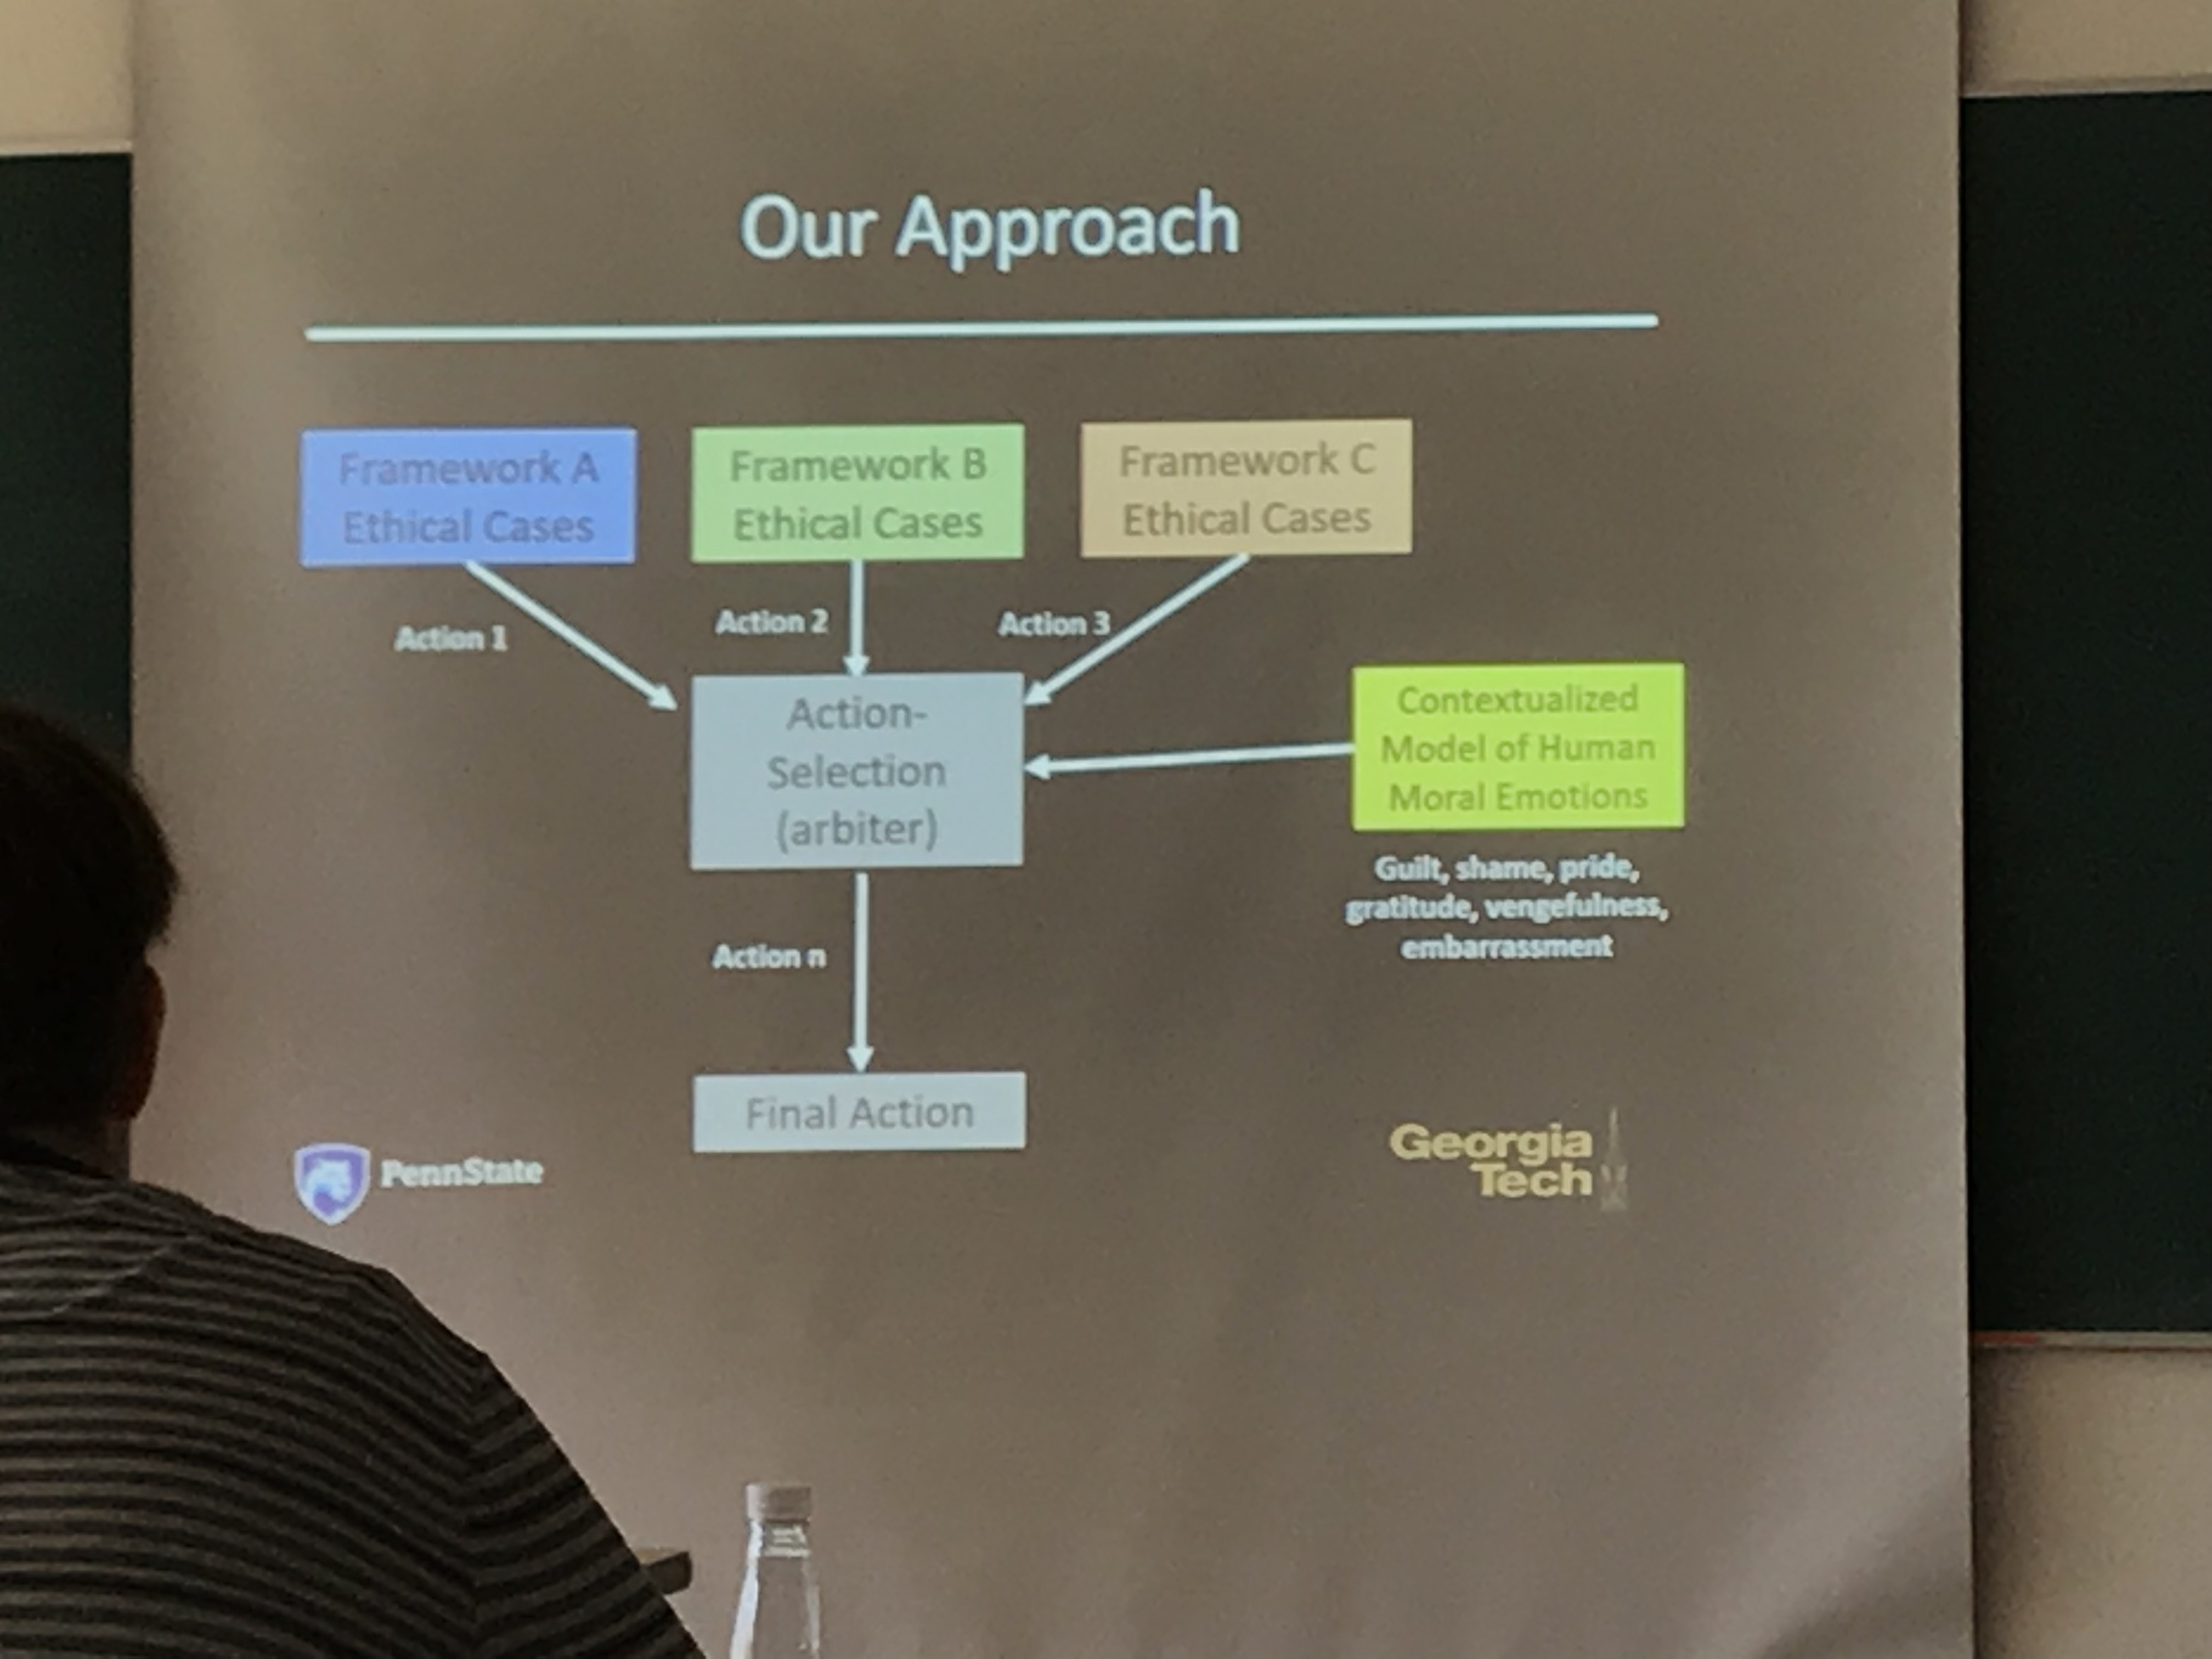
\includegraphics[width=0.5\textwidth]{kant.JPG}
\caption{Approach for ethical action arbitration and decision making.}
\label{fig:kant}
\end{figure}

{\bf Experiment 1:} Under which circumstances should one allow the opponent to win? Factors to consider: emotional state (is a child frustrated?), number of games played, age, others. \\

{\bf Experiment 2:} Pill sorting for elder care. Should the robot provide certain kinds of feedback? Say, false feedback that still encourages the person? \\


$\ra$ Survey for ethical ``answers": what do average everyday people say to do in these contexts (use AMT to collect data). Also collect ``expert opinons" from ethicists. \\


Contextualized Moral Emotions: robot retains model of emotional states of human participants; the models affect action selection. \\

Compare three action selection strategies:
\begin{enumerate}
\item Pill sorting: compare 1) always truthful (even when harsh), 2) Ethical expert recommendations, 3) Folk morality recommendations.
\item Game playing with children: 1) play to win, 2) ethical expert, 3) folk morality.
\end{enumerate}


Conclusions:
\begin{itemize}
\item Robot may need to use different ethical frameworks at different times.
\item These frameworks may not generate same action recommendations.
\item Robot may be able to use moral emotions to select best framework.
\item Possible trade-off between expert and folk opinions.
	\end{itemize}

\spacerule
\subsection{Angelica Fleury on Creating Moral Ideals in Robots from Buddhism}


{\bf Goal:} Introduce Buddhist principles for automated moral machines and contrast them from existing moral decision making methods. \\

Q: Can robots make moral decisions? \\

A: Amanda Sharkey in ``Can we program or train robots to do good?": she says no! Searle also would say no (via chinese room): strong AI can't understand their decisions, so can't make a moral decision. \\

Against Robot-Morality Skeptics:
\begin{itemize}
\item Require an assumption about a metaphysical ``self" tied to understanding. Necessary components for understanding morality.
\item Humans have a self, and this is typically sought after in robot design.
\item We ought to build a moral machine as nearly human as possible, requires claims that humans are the moral standard.
\item Objections; need for inner self as a basis for agent to have capacity fo be moral might be mistaken! Also, we should take into consideration disputes on the need for a metaphysical self.
$\ra$ Buddhists challenge the ethics of the self as something to be sought after.
\end{itemize}


Q: Should humans serve as a moral standard? \\

A: Might be the right starting point to model moral machines after, but not the standard. Our own agenda allows us to act selfishly (according to most ethical frameworks). \\

{\bf Objective:} Not to create a metaphysical moral criteria outside human influence, but instead to progress towards understanding how to make a moral machine. \\

Q: What are the necessary components for a Budhist-influenced AMA?

A: (from Danstini, Floor, Meyer 2006): 1) Autonomy (minimal sense, not Kant), 2) Emotions (need to be reciprocal, guide expression and motivation), and 3) Emotion regulation (maintain desirable emotions). \\

{\bf Approach 1:} program agents with emotions via BDI-Based agent programming language. \\
{\bf Approach 2:} program agents with emotions via ALMA (a layed model of affect). \\

$\ra$ Suggestions for modifying agents with emotions: 1) Programin initial mood to maximize empathy, 2) Appraisal (less reactionary, motivated by compassion), and 3) Coping with artifical emotion (their still triggered by if-then statements, human understandable). \\

{\bf Example:} Patient with dementia who is in need of assistance, but providers are reluctant to interact with patient due to emotional distress. Provider may neglect necessary interactions, whereas a moral machine can take into account negative emotions and recognize the need for interation and its negative emotions can be overriden. \\

Conclusions:
\begin{itemize}
\item Don't get too hung up on metaphysics of self
\item Reconsider that moral machines need to be just like humans
\item Keep emotions around but use mindfulness as a model to incorporate emotion.
\end{itemize}

\spacerule
\subsection{Simon Award Talk: Juan M Dur{\' a}n on Philosophically Analyzing Simulations}

{\bf Focus:} Come up with a systematic approach for studying computer simulations from a philosophical perspective (concentrating on two viewpoints). \\

Outline:
\begin{enumerate}
	\item First viewpoint: Problem-solving technique viewpoint
	\item Second viewpoint: Description of patterns of behaviour viewpoint: 1) historical definitions (1960-2013), 2) common topics, 3) philosophical assumptions.
	\item Philosophical implications/studies of computer simulations.
\end{enumerate}



\subsubsection{View 1: Problem Solving Techniques (PST)}

{\bf Idea:} Computer simulations are about solving a problem. \\

\ddef{PST (take one)}{(Teichroew and Lubin 1966) ``Simulation problems are characterized by being mathemaically intractable and having resisted solution by analytic methods"}

\ddef{PST (take two)}{(Humphrey 1990): ``A computer simulation is any computer implemented method for exploring the properties of mathematical models where analytic methods are unavailable."}


Common Themes from PST definitions: 1) Simulations are about finding the set of solutions to mathematical models, 2) Use of simulations is justified when analytic methods are unavailable, and 3) exploring {\it properties} of mathematical models. \\


%\subsubsection{Philosophical Assumptions}

Three key assumptions (for when to use computational simulations according to PST):
\begin{enumerate}
	\item Analytic intractibility

	$\ra$ Simulations are a tool for computing. Instrumentral role for finding results for a model. Understood as epistemically inferior to analytic methods.

	\item Implementation {\it simpliciter}

	$\ra$ Assumed that mathematical models can be directly implemented as a computer simulation. No genuine methodology mediates between the models and simulation.

	$\ra$ Simulation models are ontologically on par with mathematical models.

	\item Inherited representational capacity

	$\ra$ Simulations inherit their representational capacity of a target system from the mathematical model they implement.
\end{enumerate}

Recent paper from Bueno and Colyvan (2014) high {\it representation} as a critical piece of theories of computer simulations.

\subsubsection{View 2: Description of Patterns of Behavior (DPB)}

Again, a historical recorrd;

\ddef{DPB (take one)}{(Shubik 1960): `a simulation of a sytem is operation of a model or simulater which is the representation of a system}
\ddef{DPB (take two0}{(Bristwitle 1980) ``Simulation is a technique for representing a dynamic system by a model in order to gain information about the underlying system".}
\ddef{DPB (take three}{(Shannon 1998): ``The process of designing a model of a real system and conducting experiments with this model for the purpose of understanding the behavior of the system and evaluating various strategies for the operation of the system."}


Main idea: simulations are units of analysis in their own right (in the same way that scientific tests are). \\


Commonalities across these definitions: 1) Computer simulatins are primarily concerned with descriptions/representations of the target system, and 2) Simulations allow inferences about properties of the target system. \\


Three key assumptions (for when to use computational simulations according to DPB):
\begin{enumerate}
\item A proper methodology for computer simulations.

	$\ra$ Computer simulations become units of analysis in their own right. 

\item Own/proper representational capacity of the simulation.

\item New forms of knowledge.

	$\ra$ Capable of giving rise to new knowledge that we couldn't access through other means.
	\end{enumerate}



\subsubsection{Philosophical Implications}

Q: What can we learn about scientific explanation from these views of computer simulation? \\

A (Traditional view): mathematical model can give explanation for real-world phenomena, but not necessarily computer simulation (view from Kros 2008, Weirich 2011). \\

$\ra$ Scientific explanation: ``Simulation model does not provide an acceptable explanation of the material system" (Krohs 2008). \\

Explanation for the PST:
\begin{itemize}
	\item Analytic Interpretability
	$\ra$ ``Theoretical models need to be further analyzed or solved to provide descriptions of and predictions about the dynamics of the world they model." (Krohs).
	\item Implementation {\it simpliciter}
	\item Inherited representational capacity
	$\ra$ Since the simulation does not have explanatory input on its own and since it is limited to relating the theoretical model with the realworld phenomena, the simulation must inherit the representational capacity of the mathematical model.
\end{itemize}

Q: Do computer simulations have more to say about explanation? Or is that it? (the PST story) \\

A: Yes, explanation is better understood through the DPB \\

** Better view (from the DPB): When we explain, we don't explain the real world, {\it we explain the results of a simulation} (and hope the simulation is linked to the real world). \\

$\ra$ To solve this explanatory difficulty, we can draw a distinction between {\it knowledge} and {\it understanding}. Explanations can give us {\it understanding}, but not knowledge. \\

Key Idea: results actually shed light on the simulation itself; they help us {\it understand} the simulation. \\


Explanation for the DPB:
\begin{itemize}
	\item Scientific explanation: ``It is the simulation model, and not an exogenous mathematical model, the unity with the most explanatory relevance for the results of the simulation" (Dur{\' a}n 2017).
	\item A property methodology for computer simulations
	$\ra$ Simulations must be units of analysis in their own right.
	\item Self representational capacity of the simulation
	$\ra$ It makes possible the didentification of what can be ascribed to the world and what is an artifact of the simulation
	\item New forms of knowledge
	$\ra$ computer simulations have a {\bf genuine explanatory role} and thus ground their epistemic power.
\end{itemize}


\subsubsection{Conclusions}

Recap: two distinct viewpoints on computer simulations and their role in scientific explanation. \\

$\ra$ PST and DPB are two different theoretical frameworks about the philosophical study of simulation. PST strongly depends on mathematical models, where DPB view suggest a new methodology and epistemology of computer simulations. \\


Important note: not all definitions qualify as PST or DPB (though these two comprise most of the literature). Some others: 1) Computer simulations are arguments (Beisbart 2012), 2) COmputer simulations as unfolding the content of a well-described scenario (El Skaf, Imbert 2013). \\

Conclusion: if we can come up with well established views that unify perspectives/definitions, we can take ourselves further in this literature.

\spacerule

\subsection{Alan Wagner on The Aristotelian Robot}

{\bf Focus:} Philosophical treatment of a what it would look like to construct an Aristotelean robot. \\

$\ra$ Guiding Q: How can we construct a robot that can make use of virtue ethics? \\

$\ra$ Virtue ethics focuses on the agent, while deontology focuses on the maxim that oreitns moral action, and uitilitarian theories focus on outcomes. \\

{\bf Central Claim:} Aristotelian ethics is an optimal framework to implement for an artificial social agent. Reasons:
\begin{itemize}
	\item It can be implemented as a moral learning framework
	\item It can take into account moral psychologcal and the role of moral emotions.
\end{itemize}
%\ddef{Virtues}{Virtue is a state concerned wth choice.}

Q: Are humans by nature moral? \\
A: No! We {\it learn} to be educated by our community and our experiences. we are ``Aristotelian" humans first, later we may become Kantian, utilitarians, or nihilists. At first we are taught virtues using moral narratives and engaging their moral emotionds (moral pedagogy through narration can help teach us about morality!). \dnote{I remember reading the book of virtues as a kid!}\\

Q: How did humans become moral? \\

A: societal pressures and evolution generated the conditions for morality. Moral emotions played a critical role. \\

***Morality is a {\it societal accomplishment}. \\

Agents can learn to be moral by interacting with a community: virtues are embedded in the community. \\

Aristotle claim: core virtues are {\it quasi-universal}, and should appear in most groups: 1) self-respect, 2) gratitude, 3) courage. When a {\it conflict} arises among exemplars, core virtues are engaged. \\

$\ra$ Moral conflict can cause reflection/introspection: why is something important? Social conventions/norms unburned us from constrant moral reflection. \\

Q: How do we train a moral robot? \\

Approach: use moral narratives to teach!
\begin{enumerate}
	\item Traditionally moral training takes the form of narratives: Odysseus, Mulan, the Bodhisattva in the Jatakas.
	\item Consider the hypotheticals: ``What should X do in this situation?".
	\item Challenge: using narratives in this way requires emotional understanding!
\end{enumerate}


Aristotetlian Framework:

%\begin{figure}[h!]
%\centering
%\includegraphics[width=0.5\textwidth]{ari.JPG}
%\caption{The Aristotelian Framework}
%\end{figure}

Questions Considered:
\begin{enumerate}
	\item Are we intrinsically moral?
	$\ra$ No
	\item Moral pedagogy $\ra$ Aristotelian model
	\item Does reason move us to morality?
	$\ra$ No
	\item Can we be moral without a sense of moral persona?
	$\ra$ No
	\item Did we make ourselves moral?
	$\ra$ Yes
	\item Does the moral ``I" depend on moral narratives?
	$\ra$ Yes
	\item Does reason depend on affect to tell us what is moral?
	$\ra$ Yes
	\item Feelings required for moral emotions
	\item What's the role of phenomenology in morality?
\end{enumerate}


Conclusion:
\begin{itemize}
	\item Should be post-Cartesian and post-Turinian; we need to connect mind and body and recognize the importance of narrativity in morality.
	\item Just having emobdiment is not ehough.
	\item Cannot separate emotions from emodiement.
	\end{itemize}


\spacerule

\subsection{Himavath Jois on Should Robots be Allowed to Punish Us?}

{\bf Scenario:} an elementary school sets up a mixed robot/student team to build a bridge. In a typical team, if a student misbehaves, the teacher might scold them (put them in time out, etc.). But in this joint robot-student team, should a robot be allowed to put a misbehaving student in timeout? \\

\dbox{Guiding Q: Should robots be allowed to punish people in some circumstances?}

``Humans tend to cede decision making authority to machines in mixed robot-human teams" (Gombolary et al.). \\

Q: What is punishment for? Why is it necessary? \\

A: Punishment is critical for teaching! (See: education, sports, norms)---especially when mistakes are costly (military). \\

Q: Will humans accept punishment from a robot? And in particular, how will people respond? \\

Naive Hypothesis: People will prefer to be punished by a ronot (not advocating for this, but speculating), even when the punishment is physical! \\

Experiment: explore whether this hypothesis has merit. Setup involves a punishment device: a robotic exoskeleton capable of physical restriction as punishment for a wearer's action. \\

$\ra$ Key ethical frameworks: consequentialism, conserving autonomy, utilitarianism. \\

\begin{itemize}
	\item Consequentialist view: if the punishment leads to decreased wrongdoing, we might view it as a good thing (but, we have to consider the decrease in autonomy/pleasure of the individual)
	$\ra$ Toward autonomy: Bentham's Panoptican. Too much surveillance decreases autonomy. Would we prefer emotional control or physical control? Or just object to this loss of autonomy?

	\item Utilitarianism vs. Retributivism: Goal is to administer a punishment that decreases crime/wrongdoing. Retributive would be eye-for-an-eye.

\end{itemize}

Three scenarios:
\begin{enumerate}
	\item Scenario 1: A new house arrest device allows prisoners to live outside of prison but limits what they can do.
	\item Scenario 2: An army uses exoskeletons to maintain control over recently surrendered soldiers.
	\item Scenario 3: A world leader uses robotic exoskeletons to control a civil population and limit unrest.
\end{enumerate}

In light of these scenarios, conduct experiments that vary the type of punishment on individuals. Can receive any of: 1) no punishment, 2) verbal scolding, 3) physical restriction (through the exoskeleton). \\

$\ra$ Contrast a human initiator vs. a robotic initiator (for the punishment). \\

{\bf Preliminary Results:}
\begin{itemize}
	\item Pilot subjects presented with Godspeed survey:
	$\ra$ reported that physical punishment was very frustrating
	$\ra$ subjects that underwent robot initatied punishmen found the exoskeleten more intelligent than the human
	\item Minimal understanding of subject preferences
	\item Motivating subject to trade accuracy for speed is difficult.
	$\ra$ Currently in the process of reivisitng the methodology
	$\ra$ So this is the only beginning (but again: we're not advocating for this to happen). Just want to initiate the academic conversation, better understand human preferences about these topics.
\end{itemize}

Q: Why should we even think about this?
A: ``The machine does not isolate man from the great problems of nature but plunges him more depliny into them", Antoine de Saint-Exupery in {\it The Little Prince}. \\



\spacerule{}

\subsection{Presidential Address: Don Berkich on Underdetermination after Computation}


Q: should the philosophy of science community catch up to new computational methods? Do philosophers of science care about these advances?  (they should!) \\

\ddef{Naive View of Science}{A theory proposes (in the strong deductive sense), an experiment disposes}

One try: Observation $\implies$ $\neg$Hypothesis. But that can't be right. ``Observation" isn't propositional. \\

Note: really want to understand what we mean by ``observation" in the computational age. \\

Second try: ExperimentalObservation $\implies$ $\neg$Hypothesis. Where, ``ExperimentalObservation" is the proposition that ``specific states of affairs incompatible with the truthe of hypothesis have been experimentally observed to obtain." \\

Q: Why is this naive view of science naive? \\

A1: ExperimentalObservation is ``theory laden" (see: Duhem 1906 and Quine's Two Dogmas 1951). No putatively observational statement is observational. %Empiricists insistence on the truth of synthetic statements being reducible to the emnpirical conditions of their verification is no more sensible than their insistence that the truth of analytic statements is solely via the relationships between the meanings of terms in the statements.


A2: If ExpObs is theory laden, then falsification is ambiguous. \\

A3: If falsification is ambiguous, then scientific theory is underdetermined by the evidence for it (see: Duhemian Holism or Quinean Holism). \\

A4: Is scientific theory is underdetermined by the evidence for it, then there are no ``crucial" experiments in science. \\

A5: If no crucial experiments, then theory choice is determined by extra-scientific values.

\dbox{$\therefore$: Theory choice is driven by extra-scientific values.}

Q: What are the extra-scientific values in question? \\

Duhem A: Experimenter must display ``good sense" in choosing theory. \\

Quine A: Scientists may appeal to such principles like minimal mutilation that tend to protext math and logic. \\

$\ra$ Upshot: By good sense/minimal mutiliation/other values, naive view of science is naive insofar as it ignores the necessary role of these values in theory choice. \\

Holism: hypotheses are affected by: Science {\it and} math {\it and} Logic {\it and} Computability. \\

Q: How does the widespread deployment in the service of science affect Duhem and Quine's accounts? \\

Examples of computational methods used in science (on the side of the entailing proposition in the naive view): hurricane modeling, cellular modeling, neural modeling, ecological systems, and so on. \\

$\ra$ Computer modeling/simulations are just one half of the computational turn in the sciences. We also have data collection. \\

*These pieces are so powerful, we should update the view of science to: ComputationalObservation $\implies$ $\neg$ Hypothesis, where CompObs is the proposition that ``specific states of affairs incompatible with the truth of Hypothesis have been algorithmically inferred from vast data-troves automatically collected and classified from multiplicities of sensors. \\

Q: What is the observation when perceptual experience is no part of CompObs?\\

Discussion: Is CS epistemically privileged? Thinking about Quine's implicative view, is CS distinct from math/logic/science in some sense? \\

$\ra$ View 1: CS is science, enjoying no greater privilege than the rest of science.
$\ra$ View 2: CS is like math/logic, epistemically privileged either by being {\it a priori} or defensible as occupuyng a central commanding position in our web of belief. \\


{\bf Conclusion:} Wanted to ask: how does CS factor into our scientific theory? Is it epistemically privileged in some sense? Each possibility visited represents trouble. Moreover, computationall mediated observation may turn out to be a shaky foundation on which to build the edifice of science (as we're doing).


\dnote{And that's a wrap!}
\spacerule













% --- Bibliography ---
\newpage
\bibliographystyle{plainnat}
\bibliography{iacap}

\end{document}